\documentclass[10pt,a4paper]{article}
\usepackage[margin=0.68in]{geometry}
\usepackage{booktabs,enumitem,tikz}
\usepackage[expansion=false]{microtype}
\usepackage{iftex}
\ifPDFTeX
  \usepackage[T1]{fontenc}
  \usepackage{mathptmx}
\else
  \usepackage{fontspec}
  \usepackage{unicode-math}
  \setmainfont{Liberation Serif}
  \setmonofont{DejaVu Sans Mono}
  \setmathfont{Latin Modern Math}
\fi
\usepackage[hidelinks]{hyperref}
\usepackage{titlesec}

\setlength{\parindent}{0pt}
\setlength{\parskip}{3.5pt}
\setlist[itemize]{leftmargin=1.25em,itemsep=1pt,topsep=2pt}
\titleformat{\section}{\bfseries\large}{\thesection.}{0.45em}{}
\titlespacing*{\section}{0pt}{7pt}{2pt}
\pagestyle{plain}
\sloppy

\begin{document}

\begin{center}
{\Large\bfseries Building and Analysing a Near-Real-Time and Periodic\\
Data Warehouse for a Retail Chain}\par
\vspace{5pt}
DS3003/DS3004 - Data Warehousing \& Business Intelligence\quad$|$\quad Fall 2026\par
Ibrahim Hussain (23I-2626)
\end{center}

\section{Project overview}
This project implements a PostgreSQL warehouse for a retail chain with online and physical-store sales. Online rows arrive as a controlled stream; physical-store rows are released in hourly groups. Both pass through data cleaning, two-pass MESHJOIN enrichment and fact loading. Three independent workers (\texttt{OnlineThread}, \texttt{PeriodicThread} and \texttt{MeshJoinThread}) keep online data current without losing periodic rows during overload.

\section{Data preparation}
The source is the UCI \emph{Online Retail} dataset (1 December 2010 to 9 December 2011). Cleaning rejects missing customer IDs, non-positive quantities or prices, and cancelled invoices; it also removes exact duplicates.

\begin{center}
\begin{tabular}{lr@{\qquad}lr}
\toprule
Raw records & 541,909 & Passed cleaning rules & 397,884\\
Exact duplicates removed & 5,192 & Final cleaned records & 392,692\\
Online records & 275,154 & Periodic records & 117,538\\
\bottomrule
\end{tabular}
\end{center}

The split is by invoice, not line item. Let $h=\mathrm{int}(\mathrm{MD5}(invoice)[0{:}8],16)$. A cart is online when $h\bmod10<7$ and periodic otherwise. Online carts use store 1; physical carts use $2+(h\bmod4)$. Deterministic rules generate customer, product and supplier attributes. Periodic rows are time-sorted into 48 groups: 14 groups of 2,448 and 34 groups of 2,449. Preparation writes both master CSVs and \texttt{online\_sales\_stream.csv}; a SHA-256 manifest binds the selected files to the loaded PostgreSQL inputs.

\section{Warehouse design}
The schemas are \texttt{oltp\_online}, \texttt{oltp\_physical}, \texttt{staging\_area}, \texttt{waiting\_area} and \texttt{data\_warehouse}. The physical fact \texttt{transactions} stores one product line per cart, dimension and bridge keys, quantity, unit price, stored revenue, source identity, sales mode and processing mode. \texttt{products\_store} enforces valid product-store pairs. \texttt{fact\_sales} is a compatibility view, not a second fact.

\begin{center}
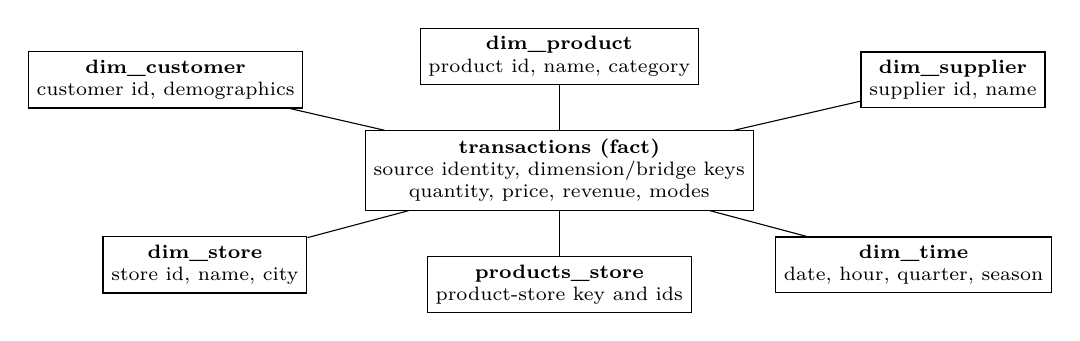
\begin{tikzpicture}[
  every node/.style={draw,align=center,font=\scriptsize,inner sep=3pt},
  line/.style={draw}
]
\node (fact) at (0,0) {\textbf{transactions (fact)}\\source identity, dimension/bridge keys\\quantity, price, revenue, modes};
\node (customer) at (-5,1.15) {\textbf{dim\_customer}\\customer id, demographics};
\node (product) at (0,1.45) {\textbf{dim\_product}\\product id, name, category};
\node (supplier) at (5,1.15) {\textbf{dim\_supplier}\\supplier id, name};
\node (store) at (-4.5,-1.2) {\textbf{dim\_store}\\store id, name, city};
\node (bridge) at (0,-1.45) {\textbf{products\_store}\\product-store key and ids};
\node (time) at (4.5,-1.2) {\textbf{dim\_time}\\date, hour, quarter, season};
\draw (customer) -- (fact);
\draw (product) -- (fact);
\draw (supplier) -- (fact);
\draw (store) -- (fact);
\draw (bridge) -- (fact);
\draw (time) -- (fact);
\end{tikzpicture}
\end{center}

\newpage

\section{MESHJOIN and loading}
MESHJOIN is a cyclic stream-relation join. The bounded stream buffer holds 1,000 rows and prioritizes online, periodic, then recovered shed rows. Each iteration reads a 500-tuple master page and moves up to 500 stream rows into hash table $H$; a FIFO queue tracks chunk order without duplicating transactions. Each chunk remains in memory for a full customer and product-master cycle. Store attributes are attached outside MESHJOIN before dimensions, the bridge, and the sales fact are written.

A 60-second simulated hour releases one periodic group. Peak mode uses 80 transactions/s and may place periodic rows in \texttt{waiting\_area.shed\_table\_physical}; non-peak mode uses 10 transactions/s and requeues them. Online rows are never shed. Source-row identities make replay idempotent. Periodic release flags and shed completion now commit atomically with the fact, while stale shed claims are recovered after a crash. Restart skips completed groups, and a database advisory lock permits only one worker. Joined online rows use the bonus durable cache and move atomically into the fact during non-peak operation.

\section{Three limitations of MESHJOIN}
\begin{itemize}
\item \textbf{Join latency:} a new chunk can wait for complete customer and product master-data cycles.
\item \textbf{Memory pressure:} overlapping chunks remain in $H$ and the queue until their scans finish; heavy arrivals can fill the stream buffer.
\item \textbf{Repeated disk I/O:} cyclic pages are reread even when few current stream rows match, limiting peak throughput.
\end{itemize}

\section{OLAP analysis and validation}
\texttt{src/queries.sql} implements all 20 required analyses: weekday/weekend top products; demographic, occupation and city analysis; monthly, quarterly and store/supplier growth; seasonal sales; cart pairs; yearly \texttt{ROLLUP}; half-year revenue; high-revenue product-days; and \texttt{STORE\_QUARTERLY\_SALES}. A materialized snapshot is also included. All aggregations use stored fact revenue.

The repaired seven-page Streamlit observatory exposes preparation, live controls, telemetry, safe relation browsing, query execution, MESHJOIN internals and system health. Automated validation compiled the Python sources, parsed 57 schema statements, 23 query statements and 5 check statements, and passed 23 unit/UI tests. The Windows runtime issues found in the supplied log were also corrected: PostgreSQL enum parameters are cast explicitly, and telemetry writes tolerate transient file locks. Every registered page rendered without an uncaught exception. A complete 541,909-row preparation reproduced all six supplied output hashes exactly.

\textbf{Observed versus pending measurements.} No PostgreSQL server was available in the repair environment, so live schema installation, full fact loading, peak shed count, non-peak recovery count and Q19 spike findings remain run-specific measurements; no values are invented. \texttt{python cli\_app.py doctor}, live telemetry and \texttt{src/checks.sql} expose the required figures on the target machine.

\section{Reflection}
The main lesson is that a warehouse load is more than copying records. Cleaning and invoice-level assignment must be reproducible; fact grain, dimension keys and stored revenue must stay consistent; and a streaming join needs explicit buffering, idempotency and crash recovery. A single protected fact table and deterministic dimensions make the analyses easier to verify.

\vfill
\footnotesize
\textbf{Data source:} Chen, D., Sain, S. L., and Guo, K., \emph{Online Retail}, UCI Machine Learning Repository, \url{https://archive.ics.uci.edu/dataset/352/online+retail}. The original download date was not present in the supplied records; the repository copy is timestamped 11 November 2026.

\end{document}
